\section{Content Blocks and Placement}
\label{sec:blocks}

The preceding rendering rules cover what can be expressed as markup inside a Text block.
This section covers what cannot.
Images and tables, which nearly every documentation chapter contains, have no tag and no substitute
in a Text block, so they have to become separate content blocks next to the text.
Placement is simple as long as an image stands between two paragraphs.
However, it becomes difficult when the image is inside a list item, a block quote, a table cell, or a
footnote, because the enclosing construct then has to be interrupted and resumed, and these
constructs can be nested.

\paragraph{One Renderer per Difficult Construct.}
The document visitor handles the simple node-to-tag mappings: text,
emphasis, headings, lists, and alerts.
Every construct that interrupts text or whose output depends on something outside the node
has its own renderer class in md2h5p's source code.
Separate renderers handle tables, images, footnotes, and links, as well as highlighted code and
questions.

\subsection{Images and Tables as Content Blocks}
\label{sec:mk_blocks}

Neither \code{img} nor \code{table} is permitted in a Text block (\autoref{tab:allowed}).
For \code{img}, there is no library that permits it in any text field.
A CSS \code{background-image} on a \code{div} does not work either, since the declaration is removed
by the sanitizer.
A relative URL inside it would not be resolved either, because the platform only rewrites the paths
of image parameters.
There is thus no way to put an image into a Text block.

\begin{figure}[H]
	\centering
	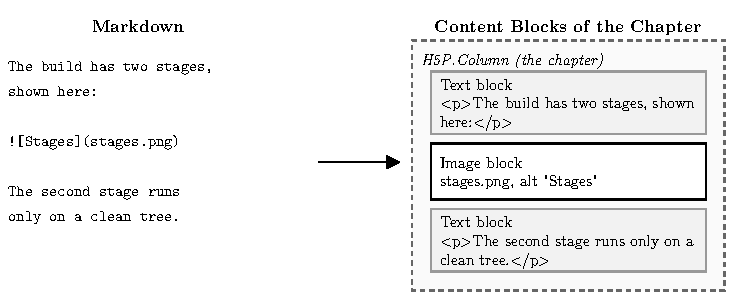
\includegraphics[width=0.9\columnwidth]{figures/block-split}
	\caption[An image splits a chapter into three blocks]{\label{fig:block_split}An image between two sentences splits the chapter into three
		content blocks: the text before it, the image, and the text after it.
		The reader sees a
		continuous page; the package holds three entries in the chapter's column.}
\end{figure}

Both constructs, however, exist as content types of their own, \code{H5P.Image} and
\code{H5P.Table}.
An image or a table therefore becomes a block after the text instead of markup inside
it.
As a consequence, a paragraph containing an image is no longer one block.
\autoref{fig:block_split} shows the simplest case: the text before the image is flushed into a Text
block, the image becomes an Image block, and the text after it starts a new Text block.
The same happens to a table in the middle of a chapter.
The reader does not notice the split, since the blocks of a column follow each other without a gap.
For an image at the top level of a chapter, this is all that is needed.

\subsection{Tables and Images}
\label{sec:mk_pseudotable}

A table without images becomes one \code{H5P.Table} block.
For example, the two-column Markdown table in \autoref{fig:regular_table} becomes a table with a
header row and two data rows.
Its HTML uses \code{table}, \code{thead}, \code{tbody}, \code{tr}, \code{th}, and \code{td}, which
are permitted in a Table block (\autoref{tab:allowed}).
The cells are also styled with borders, padding, and alignment.
The whole table remains editable as one table in the H5P editor.

\begin{figure}[H]
    \centering
    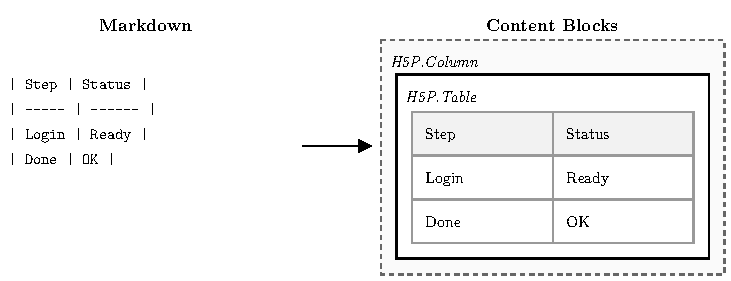
\includegraphics[width=\columnwidth]{figures/regular-table}
    \caption[A regular table as one content block]{\label{fig:regular_table}A Markdown table without images (left)
        becomes one \code{H5P.Table} block in the chapter's \code{H5P.Column} (right).}
\end{figure}

\paragraph{Images Inside Cells.}

In Markdown, a table cell may contain an image, but in a Table block it may not. A table cannot be
split around the image the way a list or a quote can.
Instead, the converter builds such a table from layout blocks.
The layout library \code{H5P.Row} places its \code{H5P.RowColumn} children side by side, and each of
them holds a vertical list of blocks, which may include Table blocks and Image blocks.
A table with an image is therefore rebuilt as one Row per table row and one RowColumn per cell.
Each cell is a vertical stack of its text as a one-cell Table block, its image as an Image block, and
any further text as another Table block.
\autoref{fig:pseudo_table} shows the structure for a two-by-two table.
The image-containing cell illustrates the split into a Table block, an Image block, and another Table block.
The result is called a \emph{pseudo-table}.

\begin{figure}[H]
	\centering
	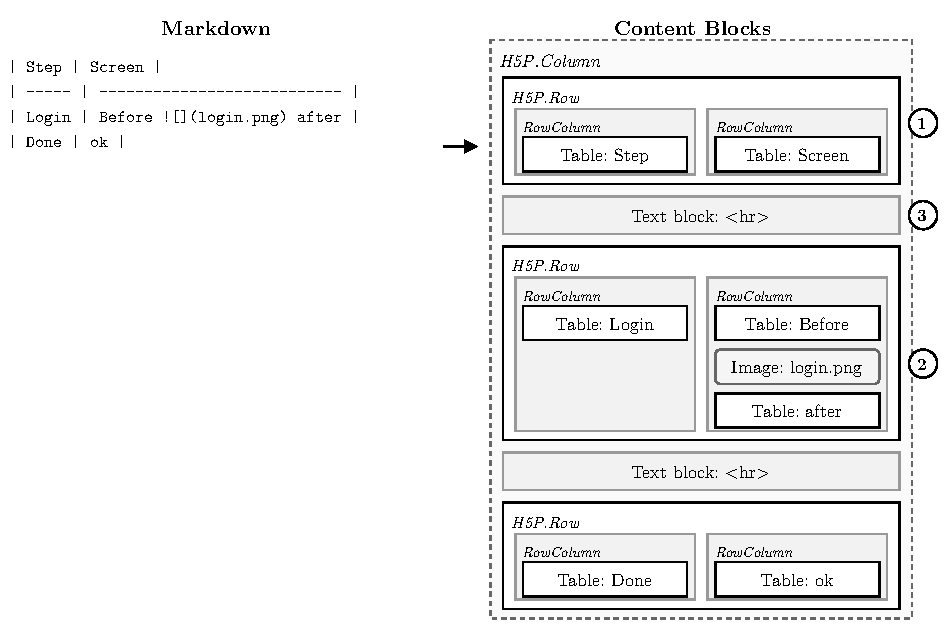
\includegraphics[width=\columnwidth]{figures/pseudo-table}
	\caption[A table with an image rebuilt as a pseudo-table]{\label{fig:pseudo_table}A Markdown table with an image, rebuilt from the layout
		library.
		Every table row becomes an \code{H5P.Row} \circled{1}, every cell an
		\code{H5P.RowColumn} holding a vertical stack of one-cell Table blocks and Image blocks
		\circled{2}, and the row boundary is a horizontal rule \circled{3} in a Text block of its own,
		drawn across the full width.}
\end{figure}

The cell's text is represented by a one-cell Table block instead of a Text block, because \code{padding} is
only available for libraries that permit \code{table} (\autoref{tab:allowed}).

The pseudo-table looks different from regular tables because its cells have no borders.
Borders around the one-cell Table blocks would frame individual text fragments rather than the
whole Markdown cell: an image can split one cell into several such blocks.
Instead, a shaded header row and full-width horizontal rules give the pseudo-table its structure.
Each rule is a separate Text block containing only \code{hr}, placed between adjacent rows.

\paragraph{Four-Column Limit.}
The pseudo-table solution works only for tables with \emph{at most four columns}, the maximum
\code{H5P.Row} permits in its \code{semantics.json}.
From five columns onward, the converter must use a regular Table block and a different fallback:
the image's alternative text becomes a placeholder in the cell, and the image itself is placed
immediately after the table.
A warning reports this displacement.
The table keeps its grid, but the image loses its position inside the cell.
\autoref{fig:pseudo_table_shot} contrasts the pseudo-table with this fallback.

\begin{figure}[H]
	\centering
	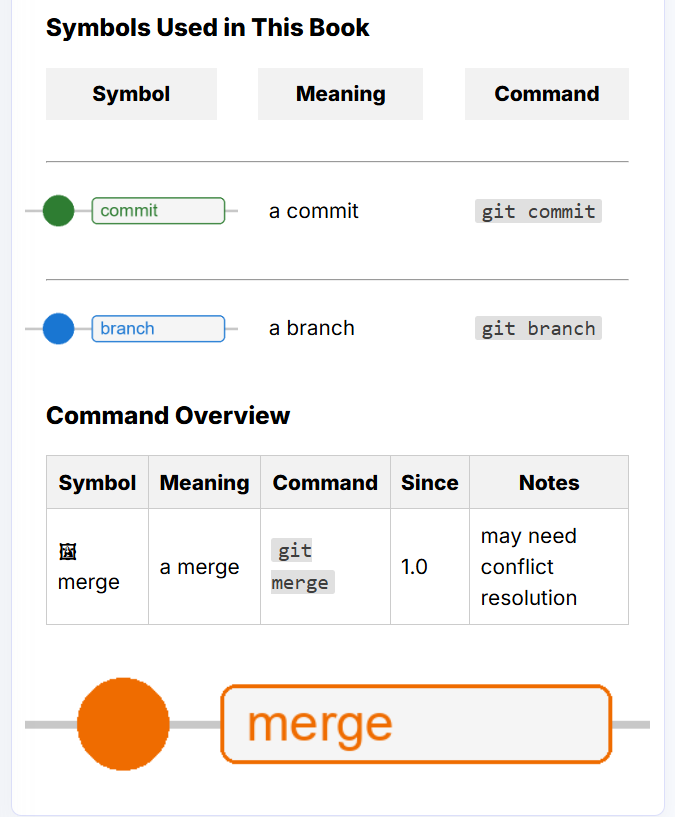
\includegraphics[width=0.75\columnwidth]{figures/screenshots/pseudo-table}
	\caption[A pseudo-table and a real table with the image lifted out]{\label{fig:pseudo_table_shot}A table with an image as a pseudo-table (top) and, above
		four columns, as a real table with the image lifted out (bottom).}
\end{figure}

The pseudo-table has several drawbacks.
In the H5P editor, it is no longer an editable table but a tree of rows and columns.
It also looks different from the other tables of the book.
Below a viewport width of 480 pixels, the layout library stacks its columns vertically, so on a phone
the table becomes a list.
Finally, it requires two additional libraries in the package.
The pseudo-table is therefore only used for tables that contain an image.

The regular table and the pseudo-table need different ways to receive an image.
This placement depends on the enclosing construct, a problem that also occurs in lists and block quotes.

\subsection{Placement Through Render Contexts}
\label{sec:bl_context}

An image needs different placement depending on what encloses it.
At chapter level, it interrupts the text; inside a pseudo-table cell, it joins the cell's vertical
stack of blocks.
Lists, block quotes, and footnotes also need to make room for images.
If the image renderer handled every enclosing construct itself, each new construct would add
another case to that renderer.

The renderer therefore keeps a stack of \emph{render contexts}.
Each context decides how to place a content block, such as a table or an image, inside its enclosing construct.
The page context is always present; rendering a pseudo-table cell pushes a cell context onto the stack.
The image renderer can then build a block independently and hand it to the innermost context for placement.

\begin{figure}[H]
    \centering
    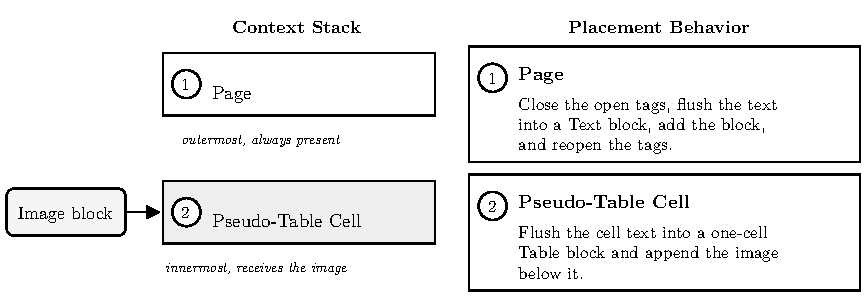
\includegraphics[width=\columnwidth]{figures/render-contexts}
    \caption[Placement of an image inside a pseudo-table cell]{\label{fig:render_contexts}The contexts
        for an image inside a pseudo-table cell, from the outermost context at the top to the
        innermost below. Each context on the left has its placement behavior shown opposite it.
        The image is handed to the cell context \circled{2}.}
\end{figure}

\autoref{fig:render_contexts} contrasts the two placement behaviors.
The page context \circled{1} closes the open tags, flushes the text into a Text block, adds the
new block to the chapter, and reopens the tags.
This produces the split shown in \autoref{fig:block_split}.
The pseudo-table cell context \circled{2} instead flushes its text into a one-cell Table block
and appends the image below it in the same column.
Further text becomes another one-cell Table block, producing the Table--Image--Table sequence
of \autoref{fig:pseudo_table}.
After the cell has been rendered, its context is removed and the previous context becomes active again.

The image renderer therefore needs no knowledge of tables.
The same mechanism also handles a table inside a block quote: the page context closes the
shaded box and reopens it after the table.
When questions were added, they were placed like any other
block, and none of the contexts had to be changed.

The page context also keeps the state of numbered lists.
Reopening an \code{ol} creates a new list, which HTML numbers from one by default.
If the third item contains an image, the fourth item would start at 1 again without an explicit start number, yielding 1, 2, 3, 1.
The page context therefore records where a list began and gives the reopened list an explicit
\code{start}.

Footnotes likewise use a separate context to interrupt and resume their numbered list.

\subsection{Footnotes}
\label{sec:bl_footnotes}

A Markdown footnote consists of a reference such as \code{[\textasciicircum{}term]} in the text
and a matching definition introduced by \code{[\textasciicircum{}term]:}.
A renderer replaces the reference with a number and displays the explanation at the end of the document.
\autoref{fig:footnotes} shows a basic example and its conversion to H5P.

\begin{figure}[H]
    \centering
    \begin{minipage}[t]{0.34\columnwidth}
        \centering
        \textbf{Markdown Source}\par\smallskip
\begin{lstlisting}[basicstyle=\ttfamily\scriptsize,frame=none,xleftmargin=0pt,framexleftmargin=0pt]
A short note explains
the term.[^term]

[^term]: This is the explanation.
\end{lstlisting}
    \end{minipage}\hfill
    \begin{minipage}[t]{0.31\columnwidth}
        \centering
        \textbf{Markdown Preview}\par\smallskip
        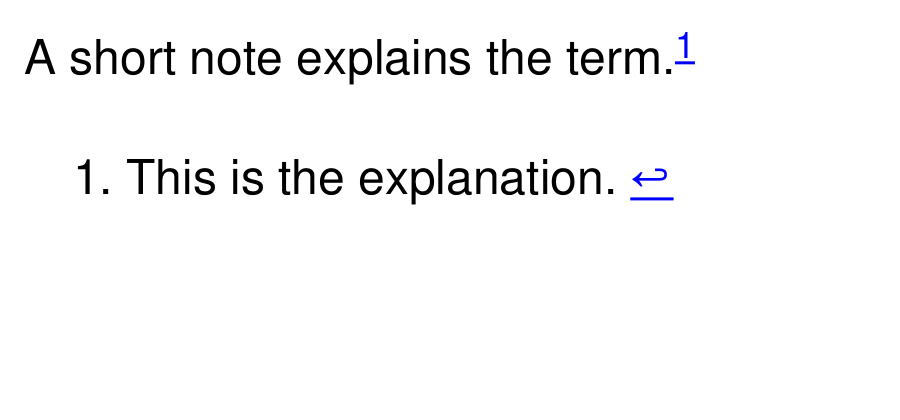
\includegraphics[width=\linewidth]{figures/screenshots/footnotes-preview}
    \end{minipage}\hfill
    \begin{minipage}[t]{0.31\columnwidth}
        \centering
        \textbf{Moodle}\par\smallskip
        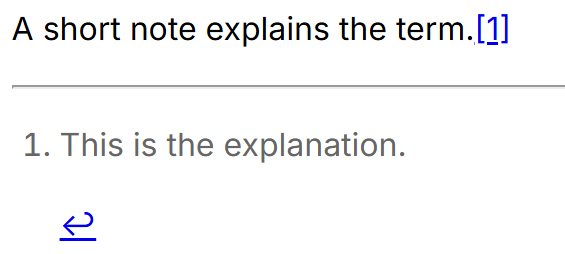
\includegraphics[width=\linewidth]{figures/screenshots/footnotes-moodle}
    \end{minipage}
    \caption[Footnotes in Markdown and Moodle]{\label{fig:footnotes}A footnote in Markdown source (left),
        in a commonmark-java HTML preview (middle), and after conversion in Moodle (right).}
\end{figure}

The converter represents the footnotes as an ordered list at the end of the chapter, separated
from the text by a horizontal rule.
References appear as bracketed numbers such as \code{[1]}, since \code{sup} is not permitted
(\autoref{tab:allowed}).
Each reference links to its list entry; a back-link returns to the reference.
An image or a table inside a footnote is placed through the same render-context mechanism.

\subsection{Links}
\label{sec:rf_anchors}

The output for a link cannot be determined from its node alone.
A Markdown link has a destination, and what the converter emits depends on where that destination
points, which in turn depends on the whole book.

\paragraph{Four Kinds of Link.}
A destination falls into one of four classes.
\circled{1} A link \emph{within the chapter}, such as \code{[the summary](\#summary)} or the wiki
link \code{[[\#Summary]]}, is emitted as an ordinary anchor.
\circled{2} A link \emph{to another chapter}, such as \code{[Setup](2\_setup.md)} with or without a
fragment like \code{\#install}, or \code{[[Setup]]}, cannot be emitted as a working link, for the
reason given at the end of this section.
\circled{3} A link \emph{to a Markdown file that is not a chapter}, such as
\code{[notes](appendix.md)}, has no target in the book, so it becomes plain text and a warning names
the file.
\circled{4} A link \emph{out of the package}, such as \code{[H5P](https://h5p.org)}, is emitted as
it is.
Whether \code{2\_setup.md} is a chapter and what title and identifier it has is unknown until
every file has been parsed.
This is why the conversion pipeline has two passes.
Wiki links are resolved as in Obsidian, by name rather than by path: an author writes
\code{[[Setup]]} instead of \code{[[2\_Setup.md]]}.
A chapter can therefore be referenced by its file name, by the file name without its number prefix,
and by its title.

\paragraph{Anchors per Chapter.}
Every heading gets an \code{id} derived from its text, so that links within the chapter can refer
to it.
Similarly, \code{id} attributes are attached to the footnote references and back-links.
However, an Interactive Book keeps several chapters in one HTML document, so ids must be unique across chapters.
Otherwise, links jump to the first element with the matching id.
To prevent a heading such as ``Summary'' from producing two elements with the same id across chapters,
the converter prefixes every id a chapter generates with \code{ch<n>-} and rewrites every
in-page link accordingly.
For example, \code{[x](\#summary)} in chapter~3 becomes \code{href="\#ch3-summary"}.
This works because the converter generates both the ids and the links.
An id written by hand in raw HTML, however, is not rewritten, since raw HTML is passed through unchanged; a Markdown link to such an anchor therefore does not work.

\paragraph{Links Between Chapters.}
\label{sec:rf_crosschapter}
The converter cannot generate working links between chapters because of how Interactive Book navigates.
It uses a URL fragment of the form
\code{\#h5pbookid=<id>}\allowbreak\code{\&chapter=<chapter-id>}\allowbreak\code{\&section=<element-id>}.
The player compares \code{h5pbookid} with the content id of the running book before it
navigates~\cite{H5P:InteractiveBook}.
The other parts of the fragment, however, are known at conversion time.
The chapter id is derived from an identifier the converter writes into the package, and the section
is the anchor's id.
The missing value is the content id, which Moodle assigns when the content is first viewed.
A package cannot choose this value, and Moodle assigns a new one when a changed package is uploaded~\cite{Moodle:Source}.
A custom library that navigates in JavaScript, as the sidebar does, would have to be added to the
content types the column accepts, which would require a modified copy of the column library.

\begin{figure}[H]
	\centering
	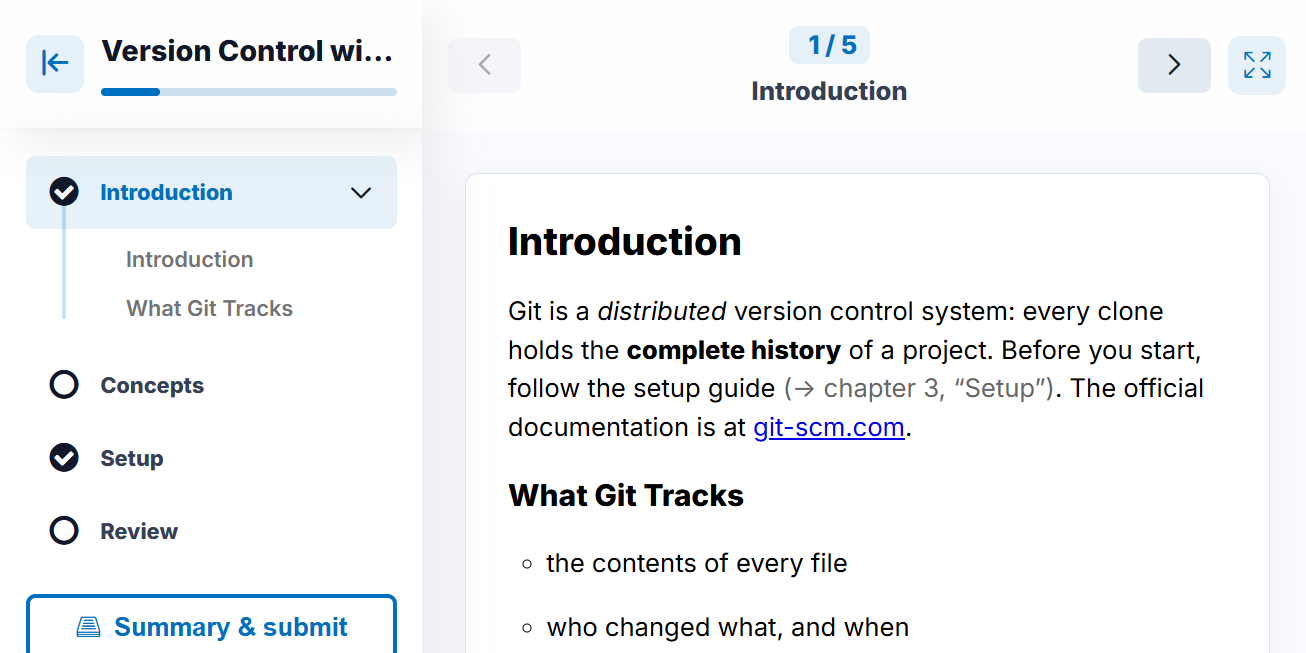
\includegraphics[width=\columnwidth]{figures/screenshots/crosschapter}
	\caption[A reference to another chapter]{\label{fig:crosschapter}A reference to another chapter as the converter renders it,
		next to the sidebar entry it points the reader to.}
\end{figure}

Instead, the converter keeps the link text and appends a muted, non-clickable note with the number
and title of the target chapter, such as ``the setup guide (\textrightarrow{} chapter 3,
``Setup'')'', and issues a warning (\autoref{fig:crosschapter}).
Since every heading is listed in the book's sidebar, which is open by default, the reader can reach
the target with two clicks.
